\documentclass[11pt,a4paper]{article}

\usepackage[margin=2.3cm]{geometry}
\usepackage[T1]{fontenc}
\usepackage{lmodern}
\usepackage{microtype}
\usepackage{amsmath,amssymb}
\usepackage{booktabs}
\usepackage{tabularx}
\usepackage{longtable}
\usepackage{enumitem}
\usepackage{caption}
\usepackage{xcolor}
\usepackage{tikz}
\usetikzlibrary{arrows.meta,positioning,fit,backgrounds}
\usepackage[hidelinks]{hyperref}

\setlist{itemsep=2pt,topsep=4pt}
\newcommand{\code}[1]{\texttt{#1}}
\usepackage{xurl}
\newcommand{\pth}[1]{\path{#1}}
\newcolumntype{L}{>{\raggedright\arraybackslash}X}

\title{Radiance Backend: Implementation Report\\[2pt]
\large From a phone video to a simulated flight, and from a phrase to a goal}
\author{Suhan --- Team Radiance, Department of Computer Science and Engineering,\\University of Moratuwa}
\date{6 October 2026}

\begin{document}
\maketitle

\begin{abstract}
This report documents the backend of the Radiance project as implemented on the lab host
\emph{intellisense08} (RTX~2080, 8\,GB): the resumable pipeline that turns a phone video into a
3D Gaussian Splat (3DGS) and flies an expert drone through it with Stanford MSL's FiGS / SOUS-VIDE,
the semantic layer that attaches CLIP and DINOv2 features to the frozen splat so that a phrase
resolves to a 3D goal, and the Galley web console that queues and inspects all of it. For every
pipeline step we state exactly which FiGS, nerfstudio or third-party call does the work. We then
report the Phase~5 comparison of four semantic variants on two scenes --- the training-free lift
localises best (0.62 and 0.63 top-1, $\approx$0.2\,m median error) and the FMGS feature field with
its paper weights the worst --- explain what the numbers mean, list concrete improvements, and
assess whether embedding semantics \emph{while training} the splat would be better than embedding
them into a frozen one. Our conclusion is that, for a simulator whose policies and courses are tied
to one fixed splat, the frozen route is the right default, and joint training is worth testing
only as a separate experiment with compressed features.
\end{abstract}

\tableofcontents
\newpage

%=======================================================================================
\section{System overview}
%=======================================================================================

The backend has three layers (Figure~\ref{fig:arch}):
\begin{enumerate}
  \item \textbf{Pipelines} (Python scripts in \code{figs/}), each a sequence of resumable steps:
        \code{figs\_pipeline.py} (capture $\rightarrow$ splat $\rightarrow$ course $\rightarrow$ expert
        flight), \code{svnet\_pipeline.py} (expert rollouts $\rightarrow$ SV-Net student), and
        \code{semantic\_pipeline.py} (teachers $\rightarrow$ lift or FMGS $\rightarrow$ feature table).
        Each step writes a completion marker with a fingerprint of the parameters it used, so an
        interrupted run restarts at the failed step and a changed parameter invalidates exactly the
        steps downstream of it.
  \item \textbf{Libraries}: FiGS / SOUS-VIDE (upstream, unmodified except documented submodule
        patches), nerfstudio~1.1.4 (\code{splatfacto}), gsplat~1.0.0, hloc + COLMAP, acados, and our
        own \code{radiance\_semantics} package.
  \item \textbf{Galley} (\code{ui/backend/galley}, FastAPI + SQLite; React frontend): a one-job-at-a-time
        GPU queue that runs the pipelines, plus fast CPU tools (course preview, splat export) and a
        long-lived CPU worker that answers semantic queries.
\end{enumerate}

\begin{figure}[ht]
\centering
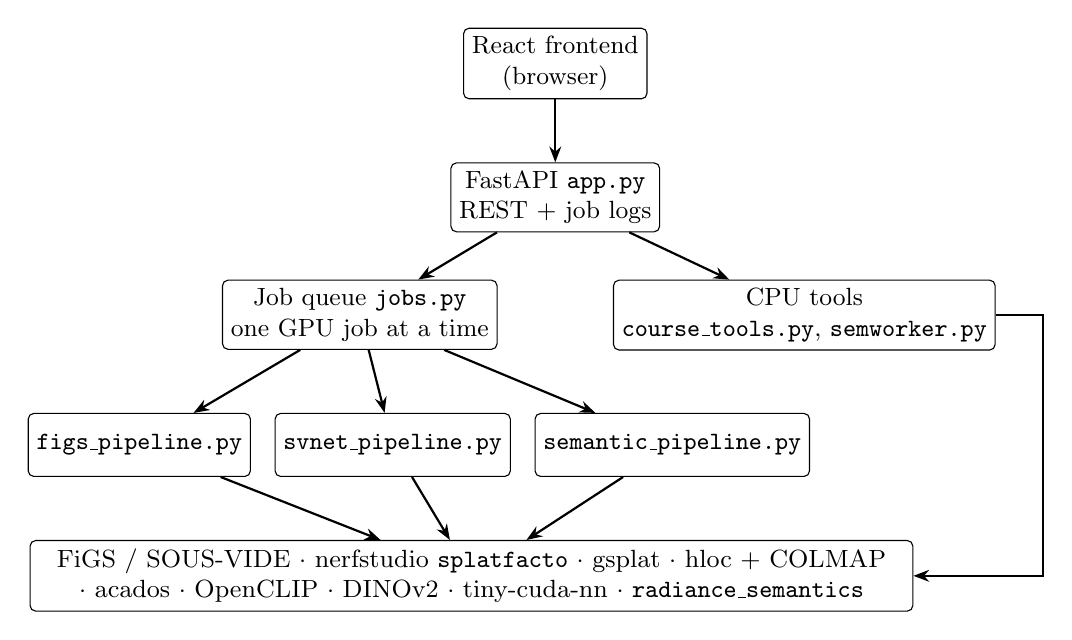
\begin{tikzpicture}[node distance=4mm and 6mm,
  box/.style={draw, rounded corners=2pt, align=center, font=\small, minimum height=8mm, inner sep=3pt, fill=white},
  grp/.style={draw, dashed, rounded corners=3pt, inner sep=5pt},
  arr/.style={-{Stealth[length=2mm]}, thick}]
  \node[box] (ui) {React frontend\\(browser)};
  \node[box, below=8mm of ui] (api) {FastAPI \code{app.py}\\REST + job logs};
  \node[box, below left=6mm and -6mm of api] (q) {Job queue \code{jobs.py}\\one GPU job at a time};
  \node[box, below right=6mm and -6mm of api] (tools) {CPU tools\\\code{course\_tools.py}, \code{semworker.py}};
  \node[box, below=8mm of q, xshift=-28mm] (fp) {\code{figs\_pipeline.py}};
  \node[box, right=3mm of fp] (sv) {\code{svnet\_pipeline.py}};
  \node[box, right=3mm of sv] (sp) {\code{semantic\_pipeline.py}};
  \node[box, below=8mm of sv, xshift=10mm, text width=11cm] (lib) {FiGS / SOUS-VIDE $\cdot$ nerfstudio \code{splatfacto} $\cdot$ gsplat $\cdot$ hloc + COLMAP $\cdot$ acados $\cdot$ OpenCLIP $\cdot$ DINOv2 $\cdot$ tiny-cuda-nn $\cdot$ \code{radiance\_semantics}};
  \draw[arr] (ui) -- (api); \draw[arr] (api) -- (q); \draw[arr] (api) -- (tools);
  \draw[arr] (q) -- (fp); \draw[arr] (q) -- (sv); \draw[arr] (q) -- (sp);
  \draw[arr] (fp) -- (lib); \draw[arr] (sv) -- (lib); \draw[arr] (sp) -- (lib); \draw[arr] (tools.east) -- ++(6mm,0) |- (lib.east);
\end{tikzpicture}
\caption{Backend layers. Every GPU-heavy action is a job in the queue; previews and semantic queries run on the CPU beside it.}
\label{fig:arch}
\end{figure}

\paragraph{Environment.} Every job runs as
\code{bash -c 'source figs\_env.sh \&\& exec \ldots'} in a fresh shell, because the pipelines need the
\code{kitchen} conda environment plus \code{ACADOS\_SOURCE\_DIR}, \code{LD\_LIBRARY\_PATH} and
\code{PYTHONNOUSERSITE=1}, which cannot be fixed inside a running process. The stack is pinned
(torch~2.1.2/CUDA~11.8, nerfstudio~1.1.4, gsplat~1.0.0, tiny-cuda-nn~2.0 built for sm\_75); additions
go in with \code{-{}-no-deps} against a frozen constraints file. Each job gets its own process group,
so cancelling reaches \code{ns-train}, COLMAP and ffmpeg children too.

%=======================================================================================
\section{Capture to flight: \texorpdfstring{\code{figs\_pipeline.py}}{figs\_pipeline.py}}
%=======================================================================================

Table~\ref{tab:figs} lists the steps and, for each, what actually does the work. Steps marked
\emph{FiGS} call upstream code unchanged; our code around them adds staging, checks, logging,
VRAM monitoring and diagnostics for known failure messages.

\begin{longtable}{@{}>{\raggedright\arraybackslash}p{1.7cm}>{\raggedright\arraybackslash}p{5.6cm}>{\raggedright\arraybackslash}p{7.8cm}@{}}
\caption{Steps of \code{figs\_pipeline.py} and the calls behind them.}\label{tab:figs}\\
\toprule
Step & What it does & What it calls \\
\midrule\endfirsthead
\toprule Step & What it does & What it calls \\ \midrule\endhead
\code{preflight} & Environment, imports, acados libraries, GPU, free disk. & Imports torch, nerfstudio, gsplat, hloc, \code{figs}, \code{acados\_template}, pycolmap, cv2, open3d; \code{ctypes} load of \code{libacados.so}; \code{nvidia-smi}. \\
\code{probe} & Inspects the source video (codec, size, HDR, VFR, frame count). & \code{ffprobe}. \\
\code{transcode} & Stages the video into \pth{gsplats/capture/<scene>.mp4} at 1920$\times$1080, fixed fps. & \code{ffmpeg -vf scale=W:H,format=yuv420p -r fps -c:v libx264 -crf 18}. (No HDR tone mapping: HLG footage stays washed out.) \\
\code{aruco} & Confirms the printed marker is visible and when; 10\,s histogram; hard-fails if the ID never appears. & OpenCV \pth{cv2.aruco.ArucoDetector} with \code{DICT\_4X4\_50}, every 2nd frame. \\
\code{config} & Writes the FiGS capture config. & \pth{configs/captures/<scene>.json}: \code{camera: null} (use SfM intrinsics), \code{extractor}: \code{num\_images}, \code{num\_marked}, \code{marker\_length}, \code{marker\_id}. \\
\code{patch} & Re-applies small fixes to hloc submodule files for the installed pycolmap API. & Edits \pth{Hierarchical-Localization/hloc/{reconstruction,extract_features}.py} only when needed. \\
\code{sfm} & Frames $\rightarrow$ structure from motion $\rightarrow$ metric alignment. & \textbf{FiGS} \pth{figs.render.capture_generation.generate_gsplat(scene)}, run with a \code{subprocess} shim that defers its final \code{ns-train} call to the next step. Inside: \code{extract\_frames} (sharp frames), nerfstudio \code{ImagesToNerfstudioDataset} (hloc SuperPoint + SuperGlue, exhaustive pairs, COLMAP), \code{extract\_positions} (ArUco \code{solvePnP} with \code{SOLVEPNP\_IPPE\_SQUARE} on frames where the marker is the only one), \code{compute\_ransac\_transform} (similarity: scale, rotation, translation), then \code{transforms.json} and \code{sparse\_pc.ply} rewritten in metres. \\
\code{train} & Trains the splat; refuses a second model per scene unless told to archive. & \code{ns-train splatfacto -{}-pipeline.model.camera-optimizer.mode SO3xR3 nerfstudio-data -{}-orientation-method none -{}-center-method none -{}-auto-scale-poses False} (+ iterations, downscale, \code{cache-images}). \\
\code{verify} & Registration rate, point cloud, exactly one model. & \code{transforms.json}, open3d on \code{sparse\_pc.ply}. \\
\code{bounds} & Camera box and recommended waypoint box; course frame. & NumPy over camera positions; course frame $=(x,-y,-z)$ of the splat frame (z down). \\
\code{course} & Validates the course file: integer cells, keyframe timing, keyframes inside the capture. & Our checks (\code{course\_int\_cells}, \code{course\_fast\_segments}, \code{course\_inside}). FiGS's \code{KF\_to\_TpFO} reads an integer cell as the previous cell's value, so integers are refused. \\
\code{simulate} & Flies the expert and renders the onboard camera. & \textbf{FiGS} \code{Simulator(scene, method, frame)}, \code{VehicleRateMPC(pilot, course, frame)} (its constructor runs \code{MinTimeSnap} and \code{TsFO\_to\_tXU}, then builds the acados MPC), \code{sim.simulate(ctl, tA, tB, x0)}, \code{generate\_videos.images\_to\_mp4}. Tracking error and pixel statistics are computed here. \\
\code{validate} & Rejects a garbage MP4 (wrong size, black frames, too short). & \code{ffprobe}, frame statistics. \\
\code{record} & Writes the run record. & \pth{SousVide/runs/<scene>_<ts>.json} (all step results). \\
\bottomrule
\end{longtable}

\subsection{Splat training}
\code{splatfacto} (nerfstudio's 3DGS) trains for 30{,}000 iterations from the SfM points. Three
choices matter downstream:
\begin{itemize}
  \item \textbf{Frames.} Orientation and centring are \code{none} and auto-scaling is off, so the splat
        lives in exactly the metric frame of \code{transforms.json}. Courses, the simulator and the
        semantic table all use that frame (the course frame flips $y$ and $z$).
  \item \textbf{Camera optimiser} \code{SO3xR3}: per-camera pose corrections learnt during training.
        Splatfacto applies them only in training mode; we apply them explicitly when we need the
        training views (Section~\ref{sec:sem}). On backroom they are worth +4.22\,dB PSNR
        (31.68 vs 27.46\,dB).
  \item \textbf{One model per scene.} FiGS loads the single model under \code{outputs/<scene>/};
        retraining archives the old one, which also changes the key that semantic tables and
        Galley's \code{.splat} cache are tied to.
\end{itemize}
Reference cost on the RTX~2080: 30k iterations in $\approx$34\,min at 960$\times$540 with a peak of
5.2\,GB (2.4\,GB with \code{-{}-cache-images cpu}). Backroom has 532{,}361 Gaussians; flightroom
379{,}684.

\subsection{Courses, preview and timing}
A course is a list of keyframes, each with a time \code{t} and a 4$\times$5 matrix of flat outputs
(x, y, z, yaw and their derivatives; empty cells are free). Galley's course editor previews it on
the CPU with \code{course\_tools.py preview}, which runs the same two FiGS calls the MPC constructor
makes (\code{MinTimeSnap}, \code{TsFO\_to\_tXU}) with the expert's \code{kT}, \code{hz}, bounds and the
frame's mass and thrust coefficient, then checks clearance against the SfM points (gap = distance to
the 5th-nearest point minus the 0.19\,m body radius) and the capture volume.

With the expert Viper (\code{kT} = 10) the file's times are only a starting guess: SLSQP re-optimises
the segment durations. We found (6~Oct) that this optimisation, run on raw durations, cannot recover
from a badly squeezed guess --- snap cost grows like $1/\Delta t^{7}$ --- and stops at the guess
while reporting success, so such a course flies as previewed (one test: 33\,m/s, 528\,\% of the
thrust limit). The editor's \emph{Add} now inserts time in proportion to distance, and the
editor, the lint endpoint and the \code{course} step flag legs faster than 5\,m/s; a re-time that
returns the file's times while breaking limits is reported as stalled.

\subsection{SV-Net student: \texorpdfstring{\code{svnet\_pipeline.py}}{svnet\_pipeline.py}}
Steps \code{rollout} (expert flights with SOUS-VIDE's data generation over the cohort's courses),
\code{observe} (per-pilot observations), \code{train\_hist} and \code{train\_comm} (the history and
command networks), and \code{deploy} (closed-loop flight of the student in the splat). The student
learns from renders of one specific splat, which is why the splat must stay frozen once a cohort
exists.

%=======================================================================================
\section{Semantics on the frozen splat: \texorpdfstring{\code{semantic\_pipeline.py}}{semantic\_pipeline.py}}\label{sec:sem}
%=======================================================================================

\begin{longtable}{@{}>{\raggedright\arraybackslash}p{1.6cm}>{\raggedright\arraybackslash}p{5.6cm}>{\raggedright\arraybackslash}p{7.9cm}@{}}
\caption{Steps of \code{semantic\_pipeline.py} (backends: \code{lift}, \code{fmgs}, \code{fmgs\_c}).}\label{tab:sem}\\
\toprule Step & What it does & What it calls \\ \midrule\endfirsthead
\toprule Step & What it does & What it calls \\ \midrule\endhead
\code{preflight} & Imports, GPU, active run, time and disk estimate. & \pth{radiance_semantics.env_check}, \code{paths.find\_scene\_run}. \\
\code{cameras} & Refined vs raw pose render check. & nerfstudio \code{eval\_setup} (\code{cameras.load\_pipeline}, run from \code{gsplats/workspace}), \code{CameraOptimizer.apply\_to\_camera} via \code{cameras.optimized\_c2w}, splatfacto rendering; PSNR. \\
\code{teachers} & 2D features per photo, cached as fp16. & OpenCLIP ViT-B/16 (LAION-2B) on a 7-scale crop pyramid (LERF), averaged onto one grid ($\approx71\times40$); DINOv2 ViT-S/14 via \code{torch.hub} (patch tokens, $\approx64\times36$). \\
\code{lift} & Blend-weighted average of teacher features onto each Gaussian. & gsplat~1.0.0 \code{rasterization} in 32-channel chunks (its backward limit); two backward passes per view give numerator and weights. \\
\code{export} & Table in Galley's \code{.splat} order. & \code{course\_tools.splat\_order}, \code{store.write\_table}. \\
\code{fmgs} / \code{fmgs\_c} & Train the FMGS feature field against the frozen Gaussians (\code{fmgs\_c}: CLIP only). & \pth{radiance_semantics.fmgs.train}: tiny-cuda-nn hash grid (split into two 12-level grids on sm\_75) + CutlassMLP heads, gsplat feature rendering, PyTorch Adam with dynamic loss scaling. \\
\code{bake} / \code{bake\_c} & Field evaluated at every Gaussian $\rightarrow$ table. & \code{fmgs.bake}, unseen rows from the lift's weights. \\
\bottomrule
\end{longtable}

\subsection{Teachers}
For each training photo, CLIP is applied to square crops at 7 scales (5--50\,\% of the short side),
each scale's grid of unit embeddings is resampled onto a common grid and the scales are averaged
(LERF/FMGS). DINOv2 supplies dense patch features that delineate objects but carry no language.
Backroom: 300 frames, 3{,}529 crops per frame, 31.5\,min, 1.3\,GB.

\subsection{Backend 1: the lift (no training)}
For Gaussian $i$ with blending weight $w_i(v,p)$ at pixel $p$ of view $v$ and teacher map $F_v$:
\[ \mathbf f_i = \frac{\sum_{v,p} w_i(v,p)\,F_v(p)}{\sum_{v,p} w_i(v,p)} . \]
Rendering is linear in the features, so the numerator is the gradient of
$\sum_p\langle \mathrm{render}(\mathbf f),F_v\rangle$ at $\mathbf f=0$ and the denominator the
gradient of $\sum_p \mathrm{render}(\mathbf 1)$: no optimisation, 3--4\,min per scene.

\subsection{Backend 2: FMGS on the frozen splat}
A multi-resolution hash grid (24 levels, 16$\rightarrow$512, $2^{20}$ entries, 8 features; built as
two 12-level tiny-cuda-nn grids because a 192-d grid does not launch on sm\_75) feeds two MLP heads
(CLIP 512, DINO 384). Each of 4{,}200 steps renders the field's outputs for the trainable Gaussians
(the 40\,\% most opaque, in frustum) from one training view at 480$\times$270 and minimises
$0.2\,\mathrm{Huber}(\text{CLIP}) + 0.8\,\|\text{DINO}\|^2 + 0.01\,\mathcal L_{\text{PA}}$. The Gaussians
never enter the optimiser and their checksum is verified. Two engineering fixes made it fit and
train on 8\,GB: PyTorch's allocator with expandable segments plus an out-of-memory retry, and dynamic
loss scaling with a norm floor in the pixel-alignment term to stop fp16 underflow/overflow inside
tiny-cuda-nn. Cost: 31\,min (F-CD) and 14\,min (F-C) on backroom.

\subsection{The table and the query}
Both backends write the same per-Gaussian table (unit CLIP and DINO rows, blend weight, geometry,
PCA colours), row $i$ = record $i$ of Galley's \code{.splat}, keyed to the checkpoint. A long-lived
CPU worker (\code{semworker.py}, JSON lines over stdin/stdout, \code{CUDA\_VISIBLE\_DEVICES=""}) keeps the
CLIP text tower and memory-mapped tables loaded and answers a query in $\approx$0.5--0.9\,s:
LERF relevancy against canonical negatives, a threshold relative to the query's own peak
($\tau = 0.55 + 0.5(\text{peak}-0.55)$), 0.1\,m voxel connected components, ranking, and an approach
point 1\,m from the object towards where the cameras looked from, clipped to the flyable box and
checked for clearance. The splat editor sends the result to a course as its final keyframe.

%=======================================================================================
\section{The Galley backend}
%=======================================================================================
\begin{tabularx}{\linewidth}{@{}lL@{}}
\toprule
Module & Role \\
\midrule
\code{app.py} & FastAPI routes: scenes, models (archive/promote), jobs and logs, courses (save, lint, preview, geometry, \code{.splat}), semantics (status, query, relevancy bytes, PCA, annotations, evaluation), videos/uploads, Drive import. Token-protected, loopback only. \\
\code{jobs.py} & The queue: strictly one job at a time in submission order, fresh shell with \code{figs\_env.sh}, own process group, live log stored in SQLite, interrupted jobs marked on restart. \\
\code{pipeline.py}, \code{svnet.py}, \code{semantics.py} & Pydantic models that validate a run and build the exact command line (\code{build\_argv}); read step markers, results and run records; status per scene (e.g. semantic tables stale when the checkpoint key changes). \\
\code{course.py} & \code{CourseTools}: runs \code{course\_tools.py} (geometry, preview, splat export) in the kitchen environment on the CPU; integer-cell and timing lint. \\
\code{semworker.py} & Starts, restarts and talks to the semantic query worker. \\
\code{configs.py} & Validated read/write of FiGS config files (courses as floats in the upstream layout, mirrored to the repo overlay). \\
\code{videos.py}, \code{drive.py} & Resumable uploads and Google Drive import of capture videos. \\
\code{tfevents.py}, \code{db.py}, \code{settings.py} & TensorBoard curves, SQLite store, machine profiles (\code{ui/machines/<host>.toml}). \\
\bottomrule
\end{tabularx}

%=======================================================================================
\section{Results: four semantic variants on two scenes}
%=======================================================================================

Query sets were annotated from the training photos and frozen in git before any query ran:
backroom 13 objects (incl. synonyms and a 3-instance class) + 3 absent objects; flightroom 16 + 3.
A query is a \emph{hit} when its top candidate's box (+0.3\,m) holds an annotated instance or its
centroid is within 0.75\,m. The query settings were fixed on a separate development set.

\begin{table}[ht]
\centering\small
\begin{tabular}{@{}llrrrrrr@{}}
\toprule
Scene & Variant & Top-1 hit & Err.\ med.\ (m) & Neg.\ FP & Neg.\ AUROC & Build (min) & VRAM (GB) \\
\midrule
backroom & L-C  & \textbf{8/13} & 0.19 & 1/3 & 0.85 & 3.0 & 7.4 \\
         & L-CD & \textbf{8/13} & 0.19 & 1/3 & 0.85 & 3.0 & 7.4 \\
         & F-C  & 6/13 & 0.32 & 1/3 & 0.80 & 13.9 & 5.8 \\
         & F-CD & 7/13 & 0.20 & 1/3 & 0.80 & 31.4 & 7.8 \\
\midrule
flightroom & L-C  & \textbf{10/16} & 0.22 & 1/3 & 0.90 & 4.4 & 2.4 \\
           & L-CD & \textbf{10/16} & 0.21 & 0/3 & 0.90 & 4.4 & 2.4 \\
           & F-C  & 8/16 & \textbf{0.11} & 0/3 & 0.81 & 11.5 & 5.1 \\
           & F-CD & 4/16 & 0.18 & 0/3 & \textbf{0.96} & 25.2 & 7.5 \\
\bottomrule
\end{tabular}
\caption{L = lift, F = FMGS; C = CLIP only, CD = CLIP + DINO (query-time DINO for L-CD, DINO loss
for F-CD). The shared teacher extraction (31--50\,min) is not included in Build. Queries take
0.54--0.9\,s on the CPU for every variant.}
\end{table}

\paragraph{What the numbers mean.}
\begin{itemize}
  \item \textbf{The training-free lift is the best localiser here.} It finds 62--63\,\% of objects
        with $\approx$0.2\,m median error, in 3--4\,min. Averaging measured features over every view
        that saw a Gaussian is hard to beat when the geometry is already good.
  \item \textbf{FMGS with CLIP alone (F-C) localises tightly but finds fewer objects}: its smooth
        field sharpens what it does find (0.11\,m on flightroom) but blurs weak, small or thin
        objects below the threshold.
  \item \textbf{FMGS with its paper weights (F-CD) fails on flightroom} (4/16) because its CLIP channel
        is spatially fragmented: for ``red cup'' the Gaussians above threshold form 61 clusters of
        $\leq$3, none large enough to count. With unit-norm 512-d CLIP targets, the 0.2-weighted
        CLIP term is about four orders of magnitude below the 0.8-weighted DINO term, so DINO shapes
        the shared hash grid and the CLIP head is noisy at Gaussian scale.
  \item \textbf{DINO at query time (L-CD) changes no hit}; it removes one false positive on an absent
        object at +50--70\,ms per query. Lifted DINO rows are smooth (neighbour similarity 0.945),
        so there is little contrast to diffuse or split on.
  \item \textbf{The failures are mostly recognition, not geometry.} In every variant, ``no candidate''
        (peak relevancy below the 0.55 floor) dominates: armchair, keyboard, floor lamp, tripod ---
        thin, low-texture or generic objects that CLIP does not single out. Wrong-object errors are
        colour + material phrases with a similar object nearby (``purple foam mat'').
  \item \textbf{Sensitivity.} Only the relevancy floor moves hits (0.50: +1--2 hits per scene but twice
        the false positives); rel\_alpha, cluster voxel and the lift's render width (480/720/960\,px)
        change nothing material --- the teacher grids are only $\approx$71 cells wide, so 480\,px already
        oversamples them $\approx$7$\times$.
\end{itemize}

\paragraph{Caveats.} 29 positive and 6 negative queries over two scenes, one training seed per FMGS
variant, ground truth placed from photos (validated at 0.09--0.42\,m against hand placements).
A third scene (GTN lab) was captured but its SfM folded two similar walls into one, so it was excluded.

%=======================================================================================
\section{What can be improved}
%=======================================================================================
\begin{enumerate}
  \item \textbf{Better teachers before better fusion.} Most misses are CLIP recognition failures. A
        larger CLIP (ViT-L/14) or a region-level model (e.g.\ SAM masks pooled into CLIP, as in
        LangSplat) would give sharper, object-shaped teacher maps; the lift would carry that
        improvement straight into 3D.
  \item \textbf{Rebalance FMGS's losses} (normalise each term by its magnitude, or raise the CLIP weight)
        and re-evaluate on a new development set; the paper weights do not transfer to unit-norm
        targets.
  \item \textbf{Per-query absence decision.} A single global floor cannot separate absent objects
        (AUROC 0.80--0.96 says the peak relevancy carries the signal); a calibrated per-scene
        threshold or a ``best match vs.\ background'' ratio test would.
  \item \textbf{Instance-aware clustering.} Voxel connected components merge touching objects and
        split thin ones; segment-level grouping (SAM in 2D, lifted) would fix both.
  \item \textbf{Capture quality.} Tone-map HDR in \code{transcode}, keep the marker visible throughout,
        avoid ultra-wide lenses, and detect SfM folds (camera yaw histogram, depth consistency)
        automatically.
  \item \textbf{Robust time optimisation.} Optimise log-durations instead of raw ones (converged in
        our test where FiGS's SLSQP stalled) --- upstream code, so proposed as a patch, not applied.
  \item \textbf{More evaluation.} More scenes, multiple seeds, the Compare view for qualitative checks,
        and the Phase~6 test of whether language-generated courses fly as well as hand-made ones.
\end{enumerate}

%=======================================================================================
\section{Assessment: semantics during splat training, or on a frozen splat?}
%=======================================================================================

\paragraph{The two routes.} \emph{Joint} methods learn a feature per Gaussian (or a feature field) in the
same optimisation that fits colour and geometry, so densification and pruning also respond to the
feature loss: Feature 3DGS~\cite{feature3dgs} distils 2D foundation features this way (with a
low-dimensional feature and a decoder to stay tractable), LEGaussians~\cite{legaussians} likewise for
language. \emph{Staged} methods fit RGB first and then fit features with geometry fixed: LangSplat
\cite{langsplat} trains compressed language features on a pre-trained scene, and FMGS~\cite{fmgs}
trains its hash-grid feature field after the Gaussians --- the route we implemented. \emph{Training-free}
methods lift 2D features onto a fixed splat by its blending weights~\cite{ludvig,occam}; LUDVIG and
Occam's LGS report results comparable to trained features at a fraction of the cost, which our
Phase~5 lift results agree with.

\paragraph{What joint training could gain.}
\begin{itemize}
  \item Geometry that follows semantic boundaries: densification could add Gaussians where a small
        object's features differ from its surroundings, which might help thin objects.
  \item A single training run instead of two, when a new scene is built anyway.
  \item Feature 3DGS reports that feature distillation can act as a mild regulariser for novel-view
        quality; the effect depends on the scene and the feature weight.
\end{itemize}

\paragraph{What it would cost in this project.}
\begin{itemize}
  \item \textbf{It breaks the frozen-splat contract.} Courses, clearance checks, the \code{.splat}
        cache and above all the SV-Net students are tied to one exact set of Gaussians. Any change
        to the semantics model would retrain the splat and invalidate cohorts; with a frozen splat,
        semantics can be rebuilt, compared and swapped at no cost to the simulator.
  \item \textbf{Risk to the photometric quality the policy trains on.} The feature loss competes with the
        colour loss for the same Gaussians and densification budget; any loss of RGB fidelity is a
        loss for SV-Net, whose input is the render.
  \item \textbf{Memory on 8\,GB.} Splat training already peaks at 5.2\,GB. Full 512+384-d features on
        500k Gaussians are $\approx$1.8\,GB of parameters, $\approx$7\,GB with Adam state --- impossible
        without compressing to a few dimensions (LangSplat's 3-d autoencoder, Feature 3DGS's decoder),
        which loses information our query uses.
  \item \textbf{Iteration speed and comparability.} The lift builds in 3--4\,min and FMGS in 12--31\,min;
        a joint run is a full 30k-iteration retrain per variant, and each variant would have
        different geometry, so a fair comparison of semantic backends would no longer be possible.
  \item \textbf{It does not address our main failure mode.} Phase~5's misses are mostly CLIP not
        recognising the object at all (peak below threshold); better geometry does not create a
        teacher signal that is not there.
\end{itemize}

\paragraph{Verdict.} For this system --- a simulator whose value is a fixed, photometrically faithful
splat that policies and courses are built on --- \textbf{embedding semantics into the frozen splat is
the better default}: it is cheaper, keeps every downstream artefact valid, allows backends to be
compared on identical geometry, and our results show the simplest frozen method (the lift) already
outperforms a trained field. Joint training is a reasonable \emph{experiment}, not a replacement: on
the planned nerfstudio branch, train a splatfacto variant with a low-dimensional semantic feature
and decoder, and compare it on the same frozen query sets \emph{and} on RGB PSNR, so that any gain in
localisation is weighed against what it does to the images the drone learns from. Improving the
teachers (Section~6, item~1) is likely to buy more than either.

\begin{thebibliography}{9}
\bibitem{fmgs} X.~Zuo, P.~Samangouei, Y.~Zhou, Y.~Di, M.~Li. \emph{FMGS: Foundation Model Embedded 3D Gaussian Splatting for Holistic 3D Scene Understanding.} IJCV 2024.
\bibitem{feature3dgs} S.~Zhou et al. \emph{Feature 3DGS: Supercharging 3D Gaussian Splatting to Enable Distilled Feature Fields.} CVPR 2024.
\bibitem{legaussians} J.-C.~Shi, M.~Wang, H.-B.~Duan, S.-H.~Guan. \emph{Language Embedded 3D Gaussians for Open-Vocabulary Scene Understanding.} CVPR 2024.
\bibitem{langsplat} M.~Qin, W.~Li, J.~Zhou, H.~Wang, H.~Pfister. \emph{LangSplat: 3D Language Gaussian Splatting.} CVPR 2024.
\bibitem{ludvig} J.~Marrie et al. \emph{LUDVIG: Learning-free Uplifting of 2D Visual Features to Gaussian Splatting Scenes.} 2024.
\bibitem{occam} J.~Cheng et al. \emph{Occam's LGS: An Efficient Approach for Language Gaussian Splatting.} 2024.
\bibitem{lerf} J.~Kerr et al. \emph{LERF: Language Embedded Radiance Fields.} ICCV 2023.
\end{thebibliography}

\end{document}
